\chapter{Modelado y conjuntos de datos}\label{cap:arquitecturayconjuntosdedatos}

En este capítulo se detalla la metodología que se utilizó en la presente tesis para resolver ZSD. Específicamente, se explayan las distintas etapas, se presentan los conjuntos de datos utilizados y se desarrolla como puede evaluarse el rendimiento de los modelos de ZSD Y GZSD en estos conjuntos de datos.\\

En la actualidad la arquitectura más utilizada por la comunidad científica para resolver el problema de ZSD, es utilizar el espacio que forman modelos como Word2Vec~\cite{mikolov2013distributed} o GloVe~\cite{pennington2014glove} para transferir el conocimiento de las clases vistas a las invisibles. Luego de analizar los distintos artículos (ver \autoref{ssec:trabajosrecientesenzsd}), y basándonos en la complejidad del modelo y sus resultados, se decidió apoyarse en el trabajo de Bansal \etal~\cite{bansal2018zero} para abordar el problema de ZSD. En las siguientes secciones se abordaran las distintas etapas y los detalles de la arquitectura.


\section{Modelado}\label{ssec:preprocesamiento} 
Antes de detallar el entrenamiento de la arquitectura, es necesario explayar como se modifican los datos para poder ser utilizados. Cada dato de entrenamiento consiste de una imagen y un conjunto de cuadros delimitadores con el nombre de la clase del objeto que se encuentra dentro del cuadro. El objetivo de esta etapa es generar por cada imagen un conjunto de puntos en el espacio visual y semántico que corresponde a cada cuadro. Por un lado, se recortan los cuadros de la imagen $x_i$ y se reescalan a un tamaño fijo, por ejemplo 224$\times$224. Luego se utiliza una CNN pre-entrenada como VGG16~\cite{simonyan2014very} para generar los vectores visuales de cada cuadro. La salida de este paso es:

\[B_i = [\phi(b_0),...,\phi(b_k) \mid \phi(b_i) \in \mathbb{R}^{D_1}]\] 

Donde $B_i$ son todos los vectores de características visuales de la imagen $x_i$.

Por otro lado, cada cuadro se asocia con el vector semántico de la clase que tiene asignado, que se puede obtener con modelos de vectores de palabras previamente entrenados, como Word2Vec~\cite{mikolov2013distributed} o GloVe~\cite{pennington2014glove}. Dando como resultado:

\[W_i = [w_0,...,w_k \mid w_i \in \mathbb{R}^{D_2}]\]

Donde $W_i$ son los vectores semánticos asociado a cada cuadro. En la \autoref{fig:arqutectura} se ejemplifica los pasos mencionados anteriormente.\\


En la inferencia se quiere predecir la clase a la que pertenece cada cuadro delimitador en una imagen, para esto, se computa el vector visual $\phi(b_i)$ obtenido por una CNN como VGG16~\cite{simonyan2014very}, y luego utilizando la matriz de proyección $W_p$ (que nos permite pasar del dominio visual al semántico, ver \autoref{ssec:formalizaciondezsd}), calculamos el vector semántico asociado al vector visual. Por último se calcula la similitud coseno entre el vector semántico obtenido y el de todas las clases que se quiere evaluar, asignándole a esa propuesta la que obtenga un mejor puntaje. La \autoref{fig:arquitectura_prueba} muestra la arquitectura empleada en la etapa de inferencia.

\begin{figure}[H]
	\centering
	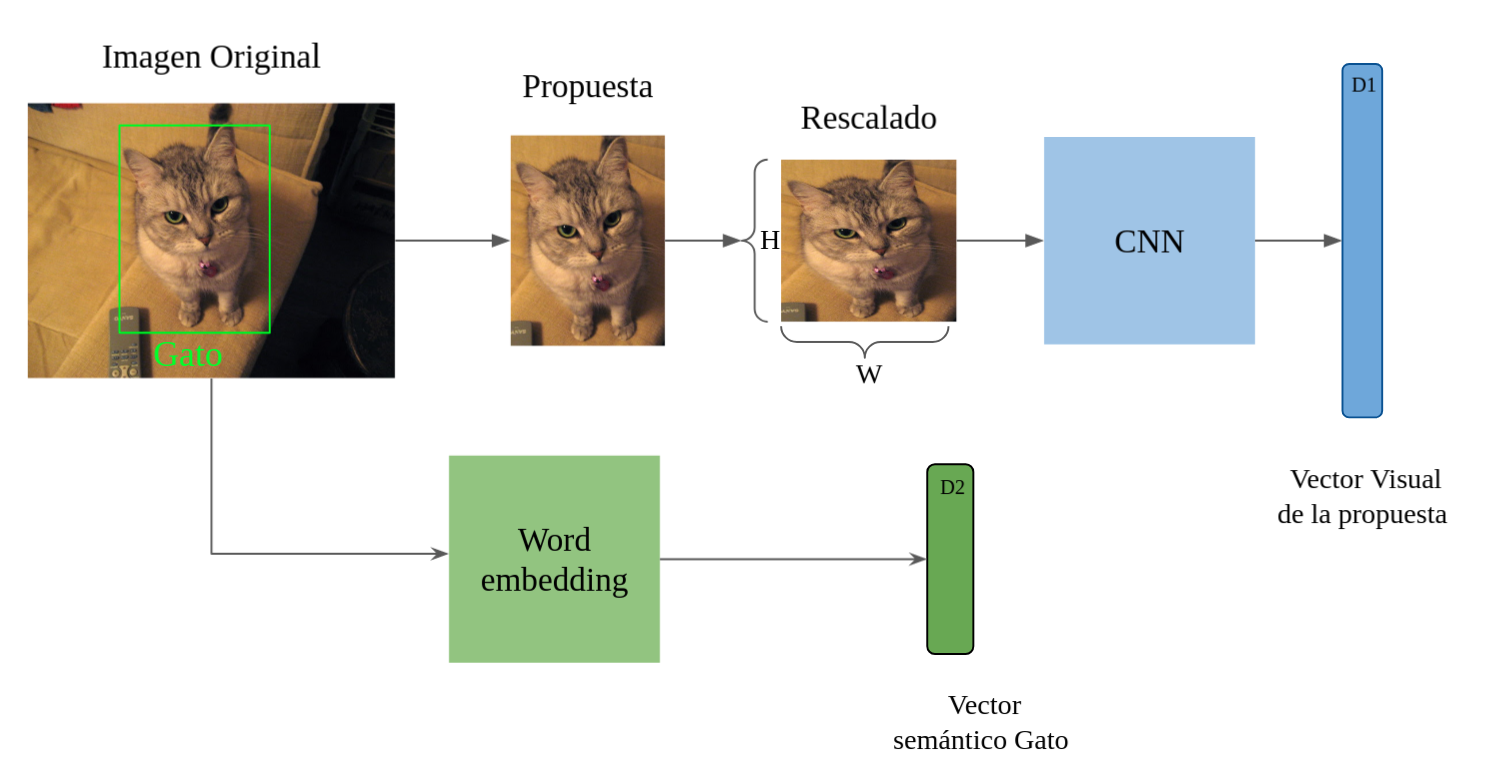
\includegraphics[width=0.9\textwidth]{img/arquitectura.png}
	\caption{Esquema del pre-procesamiento de las imágenes y de como se obtienen los vectores semánticos y visuales.}
	\label{fig:arqutectura}
\end{figure}

\begin{figure}[H]
	\centering
	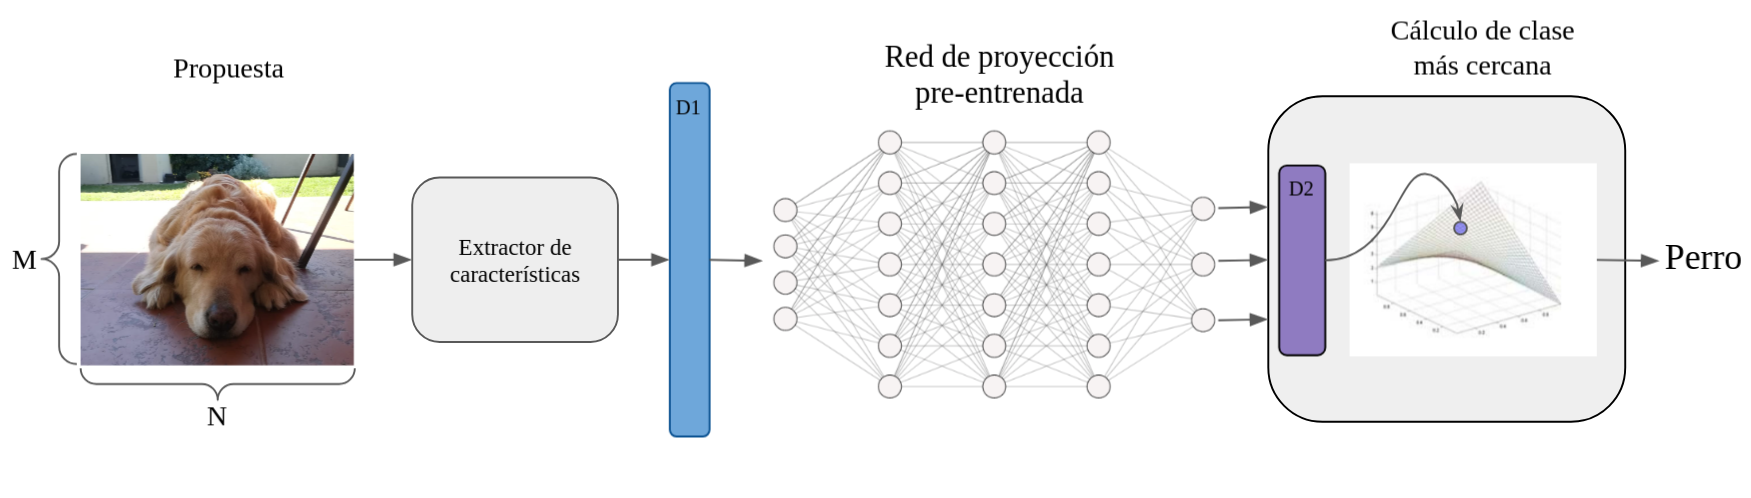
\includegraphics[width=0.9\textwidth]{img/arquitectura_prueba.png}
	\caption{Arquitectura propuesta para inferir los vectores semánticos (por ende a la clase que pertenece un cuadro delimitador) a partir de un vector visual.}
	\label{fig:arquitectura_prueba}
\end{figure}

\section{Entrenamiento del modelo}\label{ssec:entrenamiento}

\subsection{Función de costo}

Utilizamos el espacio semántico (${R}^{D_2}$) para calcular una medida de similitud entre las proyecciones de $\phi(b_j) \in B_i$ y los vectores semánticos $w_j \in W_i$. Luego, para entrenar la proyección $W_p$, que nos permite transformar un vector del espacio visual a uno del espacio semántico, definimos una función de costo, que imponga la restricción que el puntaje de la similitud de un cuadro delimitador, con su clase verdadera, debe ser más alto que el de otras clases. Por ejemplo, la proyección de un cuadro que tiene un ``perro'', tiene que estar lo más cerca posible del vector semántico ``perro'', y a su vez lejos de cualquier otro vector semántico como ``gato'' o ``auto''.

Utilizaremos la función de costo definida por \cite{bansal2018zero}~Bansal \etal: 

\[\mathcal{L}(\psi_i, w_i) = \sum_{j \in \mathcal{S}, j\neq i} max(0, m - S_{ii} + S_{ij})\] 
donde $m$ es el margen máximo, y $S_{ij}$ es la similitud entre la proyección visual $i$-$esima$ y el vector semántico $j$-$esimo$. 

Para comprender mejor esta función supongamos un margen máximo de 1, y que para todo $S_{ij}$ se cumple $0 < S_{ij} < 1$. Si la similitud entre la proyección y su vector semántico ($S_{ii}$) es cercano a 1, la función sólo dependen de los $S_{ij}$, con $j \neq i$, cuando estos valores se acercan a 0 la función de costo se minimiza, y cuando aumentan la función de costo también lo hace. Por otro lado, si la similitud $S_{ii}$ es aproximadamente 0, estaríamos penalizando la función sin importar los $S_{ij}$, pero si estos aumentan la función de costo crecerá a la par de ellos. \\


También se agrega una función de costo de reconstrucción ($\mathcal{L}_r$) como sugiere Kodirov \etal~\cite{kodirov2017semantic}. En esta función se utilizan las características del cuadro delimitador proyectadas para reconstruir los vectores visuales originales, y calcular la pérdida de reconstrucción como la distancia $L2$  entre el vector reconstruido y el original:
\[\mathcal{L}_r = \Vert{\phi(b_i) - \psi_iW_p^T}\Vert^2 \] 
Luego, definimos $\lambda$ como un coeficiente de ponderación que controla la importancia del primer y segundo término, que corresponden a las pérdidas de proyección y reconstrucción, respectivamente. Por lo cual, la función de perdida total es: 
\[\mathcal{L}_t = \lambda \mathcal{L} + (1-\lambda) \mathcal{L}_r \]

Es común que en la detección de objetos se incluya una clase de fondo, para obtener un detector robusto que pueda discriminar eficazmente entre objetos de primer plano y objetos de fondo. En ZSD, esto no es un problema trivial, ya que no se sabe si un cuadro de fondo incluye elementos como cielo, tierra, bosque, etc. o una instancia de una clase de objeto invisible. En muchos trabajos \cite{rahman2018zero, bansal2018zero} se proponen distintas técnicas para abordar este problema, pero no presentan mejoras en evaluaciones cuantitativas. Es por esto que no se incluye una arquitectura que discrimine cuadros de fondos.

\section{Conjuntos de datos} \label{sec:conjuntosdedatos}

En la actualidad no existe un conjunto de datos pensado para evaluar ZSD, es por esto que se tiene que adaptar otros conjuntos de datos para poder medir el rendimiento de los modelos. Otra posibilidad es crear un conjunto de dato sintético que emule imágenes de la vida real para ser utilizados en ZSD.

\subsection{Common Objects in Context (COCO)}\label{ssec:commonobjectsincontext}

COCO es una base de datos que tiene como objetivo ayudar en la investigación de detección de objetos, posee varias características como segmentación de instancias, subtítulos de imágenes y localización de puntos clave de personas. Este conjunto de datos contiene 80 tipos de objetos o  clases (65 para COCO 2014), con un total de 2.5 millones de instancias etiquetadas en 328.000 imágenes. La \autoref{fig:ejemplo_coco} muestra algunas imágenes que forman parte del conjunto COCO.

\begin{figure}
	\begin{center}
		\centering
		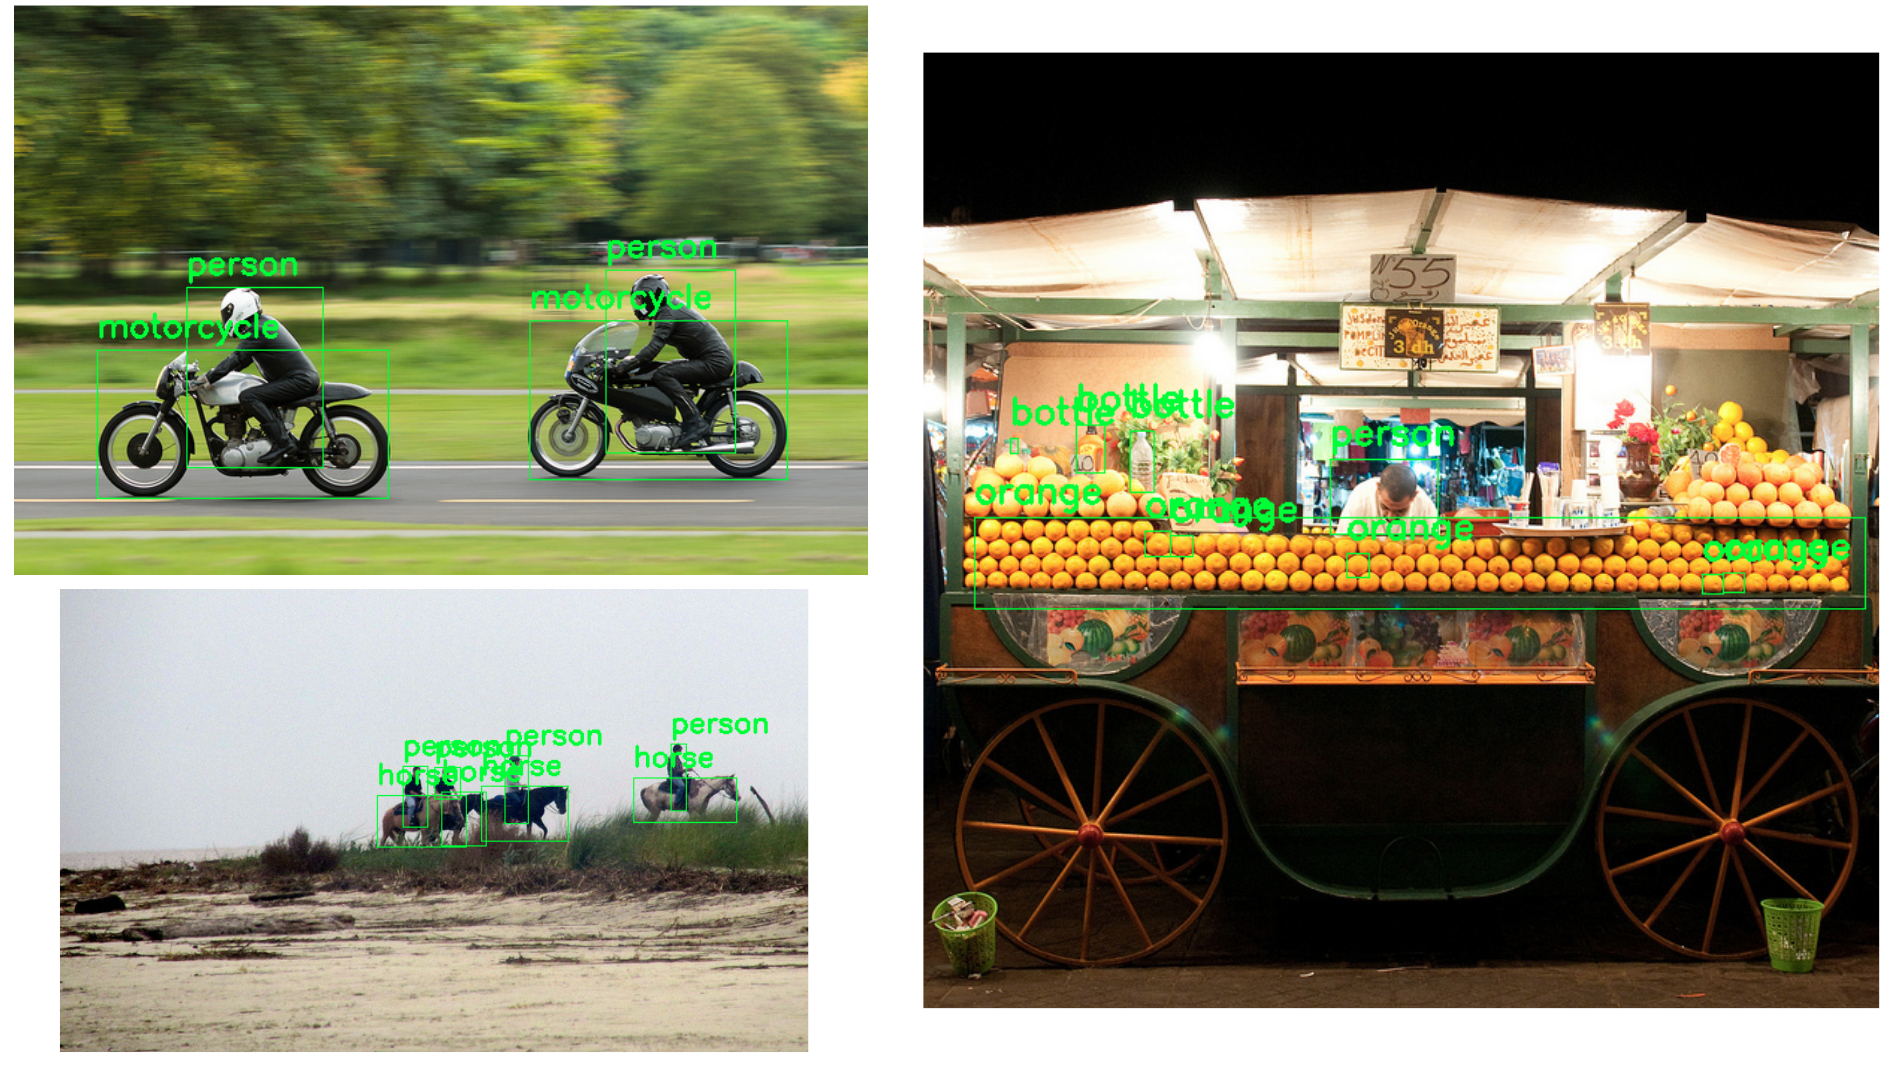
\includegraphics[width=1\textwidth]{img/coco_ejemplo.png}
		\caption{Ejemplos de imágenes del conjunto de datos COCO.}
		\label{fig:ejemplo_coco}
	\end{center}	
\end{figure}

La gran cantidad de instancias de objetos y de categorías, resulta en un conjunto ideal para entrenar y evaluar modelos de ZSD. Además, la mayoría de la imágenes constan de una gran cantidad de objetos, a diferencia de conjuntos como Visual Genome~\cite{krishnavisualgenome}. Estas tipo de imágenes generan un contexto en el que varios objetos se relacionan y se superponen, emulando de una mejor manera situaciones de la vida real. 

En este trabajo se utilizan las imágenes de entrenamiento del conjunto COCO 2014 e imágenes del conjunto de validación para realizar las pruebas de ZSD.

\begin{figure}
	\begin{center}
		\centering
		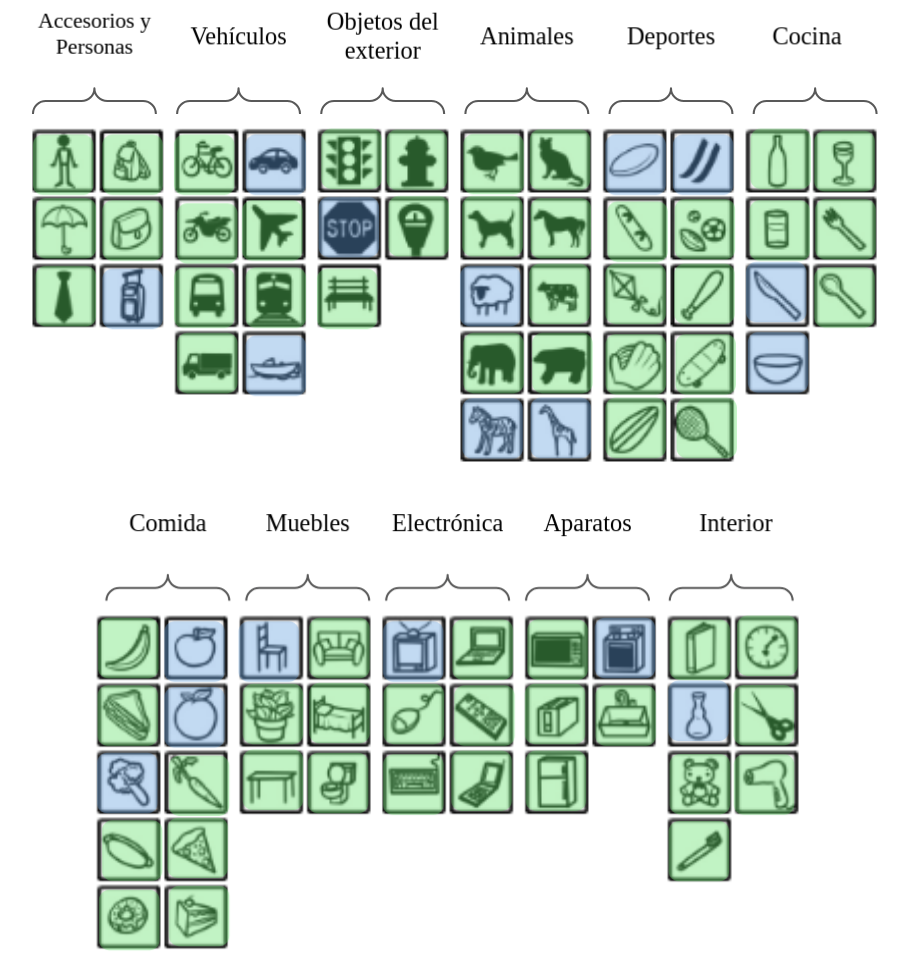
\includegraphics[width=1\textwidth]{img/data_set.png}
		\caption{División de las clases para entrenamiento (verde) y pruebas (azul).}
		\label{fig:data_set}
	\end{center}	
\end{figure}

Como COCO no provee una separación de los datos para evaluar modelos de ZSD, es necesario crear una forma de dividir las clases en vistas e invisibles. Esta separación resulta de suma importancia, ya que se debe cumplir que para todo objeto del conjunto prueba, exista otro de aspecto similar que este presente durante el entrenamiento. Además, no se puede encontrar ningún objeto de prueba en los datos de entrenamiento. Para esto, se aprovecha que COCO tiene agrupadas las clases por ``Clases superiores'' donde se agrupan objetos que tienen alguna relación. Por ejemplo, la clase superior animales contiene las clases zebra, perro, gato, etc. Por cada uno de estos grupos se elige de forma aleatoria un 70\% de clases para entrenamiento y un 30\% para pruebas. Es decir, 47 y 18 clases, respectivamente, de un total de 65 clases de COCO 2014. En la~\autoref{fig:data_set} se puede observar el resultado de esta división. Por último, se eliminaron todas las imágenes de entrenamiento que contengan al menos una instancia de las clases de prueba. Esto resulta en 42.564 imágenes, con 261.258 instancias de entrenamiento, y 3.008 imágenes con 10.878 instancias de prueba. 

Bansal \etal~\cite{bansal2018zero}, divide el conjunto de datos de manera similar, utilizando la misma cantidad de clases para las etapas de prueba y entrenamiento. Pero la diferencia radica en que utiliza los vectores densos de palabras para agrupar las clases, utilizando la  similitud coseno entre los vectores como métrica. Por último, elige de forma aleatoria las clases visibles e invisibles de cada grupo. En este trabajo también se utiliza esta separación para logra una comparación de modelos más justa.


\subsection{CIFAR-ZSD} \label{ssec:cifarzsd}

\begin{figure}[]
	\begin{center}
		\begin{subfigure}{.3\textwidth}
			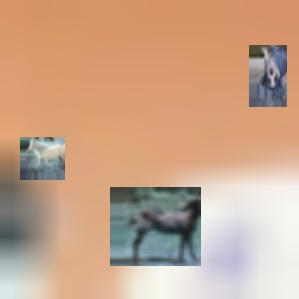
\includegraphics[width=1\textwidth]{img/cifar-zsd-test400.jpg}
			\label{fig:ex1}
		\end{subfigure}
		\begin{subfigure}{.3\textwidth}
			
\includegraphics[width=1\textwidth]{img/cifar-zsd-test379.jpg}
			\label{fig:ex2}
		\end{subfigure}
		\begin{subfigure}{.3\textwidth}
			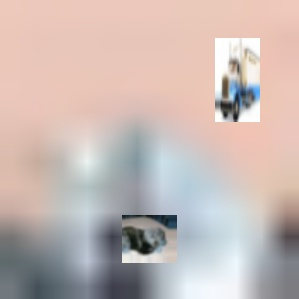
\includegraphics[width=1\textwidth]{img/cifar-zsd-test283.jpg}
			\label{fig:ex3}
		\end{subfigure}
		\caption{Ejemplos de imágenes del conjunto de datos CIFAR-ZSD.}
		\label{fig:CIFAR-ZSD}
	\end{center}
\end{figure}

COCO puede resultar pesado en término computacional. Para solucionar esto se creó un conjunto de datos sintético basado en CIFAR-100 dataset, el cual denominamos CIFAR-ZSD. Este consta de imágenes localizadas, rotadas y re-escalada aleatoriamente con un fondo de otra imagen (algunos ejemplos se pueden ver en la \autoref{fig:CIFAR-ZSD}). Con esto se intenta simular imágenes reales en la cual un objeto puede aparecer con distintos aspectos y escalas. Este conjunto esta dividido de tal forma que ninguna instancia de prueba  aparezca en el conjunto de entrenamiento.

Aunque este conjunto resulta muy útil para hacer pruebas de modelos, no es bueno para reportar métricas reales, pero en combinación con COCO, que si lo es, facilita los experimentos a realizar.


\subsection{Definición de métricas} \label{ssec:definiciondemetricas}
Entre los diferentes conjuntos de datos anotados utilizados por los desafíos de detección de objetos y la comunidad científica, la métrica más común utilizada para medir la precisión de las detecciones es el  \textit{Mean Average Precision (mAP)}, seguida por \textit{Recall}. Un dificultad que tienen los modelos de detección a diferencia de los de clasificación, es el calculo de estas métricas ya que no es trivial definirlas. Además, no existe una implementación estándar y pública para calcularlas, y aquellas implementaciones públicas están muy encapsuladas en el código, y resulta muy difícil adaptarlo para medir rendimientos de modelos propios. Como ya se mencionó anteriormente, el código de Bansal \etal~\cite{bansal2018zero} no esta disponible, por este motivo fue necesario encontrar alguna implementación de estas métricas. A partir de estas búsqueda se encontraron varias opciones, sin embargo los resultados variaban mucho de un código a otro. Esto se debe a la falta de consenso en diferentes trabajos e implementaciones de AP, que es un problema al que se enfrentan las comunidades académicas, tal como se plantea en artículo de Padilla \etal~\cite{padilla2020survey}. Además, \cite{padilla2020survey} propone una definición y un código para estandarizar las métricas, de manera que se puedan comprar distintos modelos de una forma ``justa''. Por estos motivos decidimos utilizar este trabajo y su implementación para calcular nuestras métricas, aunque los resultados no den exactos a los reportados por Bansal \etal~\cite{bansal2018zero}.\\

Ahora definamos las métricas, basándonos en el trabajo \cite{padilla2020survey}. Primero es necesario definir algunos conceptos:
\begin{itemize}
    \item Intersección sobre unión (\textbf{IoU}): es un término utilizado para describir el grado de superposición de dos cuadros. Cuanto mayor sea la región de superposición, mayor será el IoU, la \autoref{fig:iou} ilustra este concepto.
	\item Falso negativo (\textbf{FN}): Para un cuadro delimitador verdadero no se obtuvo ninguna detección en absoluto, o una propuesta tiene IoU $> umbral$ con algún cuadro verdadero y no se predijo correctamente la clase.
	\item Falso positivo (\textbf{FP}): Una propuesta predijo correctamente la clase de un cuadro delimitador verdadero pero el IoU $< umbral$, o es un predicción duplicada, es decir, ya se marco otra con mayor IoU como \textbf{TP}, o se detecto un objeto inexistente con IoU $< umbral$ para todo cuadro verdadero.
	\item Verdadero positivo (\textbf{TP}): Una propuesta predijo correctamente la clase y obtuvo un IoU $> umbral$ con algún cuadro verdadero.
	\item Verdadero negativo (\textbf{TN}): Esto sólo tiene sentido si se quisiera medir propuestas que no tienen un IoU $> umbral$ con todos los cuadros verdaderos, y además se predijo como clase de fondo. Pero en este trabajo no es utilizada.
\end{itemize}
El umbral por lo general es 0.5, pero se puede cambiar para exigir que las propuestas tenga una mayor superposición con los objetos en la imagen.\\

\begin{figure}
	\begin{center}
		\centering
		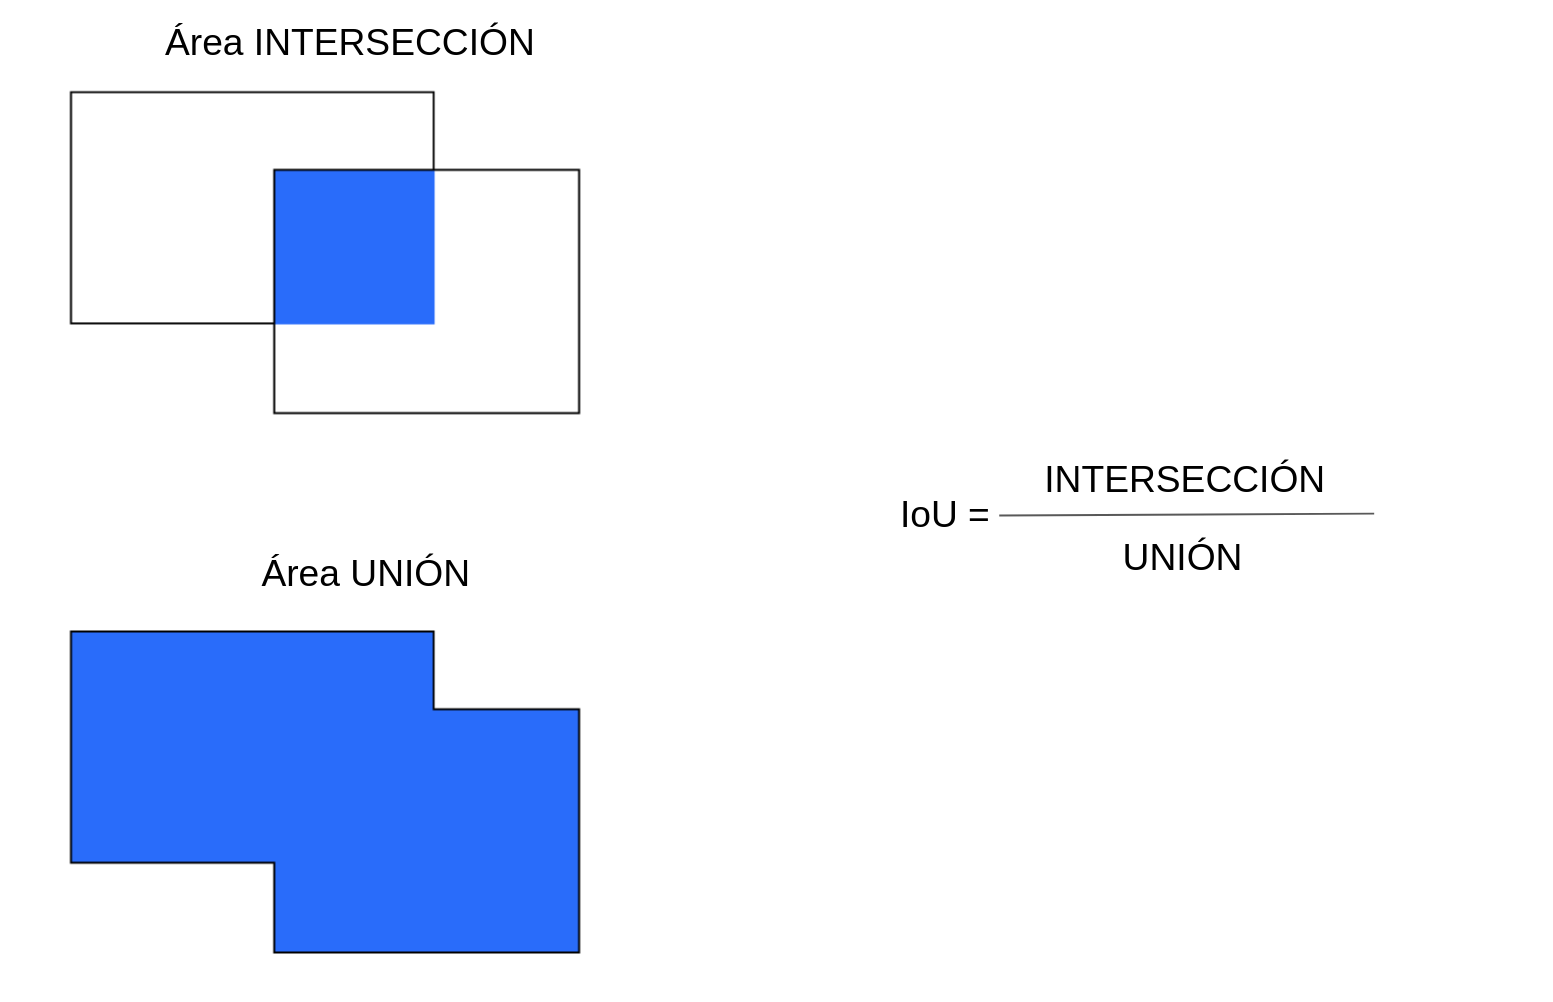
\includegraphics[width=0.8\textwidth]{img/iou.png}
		\caption{Intersección sobre unión de dos cuadros.}
		\label{fig:iou}
	\end{center}	
\end{figure}

La \textit{Recall}, también conocida como exhaustividad, mide la probabilidad de que los objetos anotados en la imagen se detecten correctamente, y viene dado por: 

\begin{equation}
	\label{eqn:recall}
	Recall =\frac{TP}{FN+TP}
\end{equation}

En otras palabras la \textit{recall} contabiliza cuantos objetos se detectaron correctamente de todos los anotados en una imagen.\\

El trabajo de Bansal \etal~\cite{bansal2018zero}, define \textit{Recall} de la siguiente manera: 
\begin{center}
	\textit{``Un cuadro delimitador predicho se marca como verdadero positivo solo si tiene una superposición de IoU mayor que un cierto umbral $t$ con un cuadro delimitador existente en la imagen y no se ha asignado ningún otro cuadro delimitador de mayor confianza al mismo cuadro. De lo contrario, se marca como falso positivo.''}\\
\end{center}

Según esta definición solo se tienen en cuenta los objetos que tuvieron al menos una propuesta con un IoU $> 0.5$, y el resto quedan fuera del cálculo de esta métrica. Esto genera una diferencia enorme entre los resultados calculados con esta definición y con los obtenidos usando la \autoref{eqn:recall}. Con el objetivo de poder comparar los resultados con otros modelos, en este trabajo se calcula la \textit{Recall} de ambas formas. 

Bansal \etal~\cite{bansal2018zero} además calcula una variación denominada \textit{K@Recall}, donde sólo se tienen en cuentan las \textit{K} mejores propuestas basándose en la confianza de la predicción y el resto son descartadas.\\


\textit{AP}, es una métrica popular para evaluar la precisión de los detectores de objetos mediante la estimación del área bajo la curva (AUC), que viene dada por la relación de la \textit{precisión} y la \textit{recall}. Donde la precisión consiste en medir el proporción de predicciones positivas correctas entre todas las predicciones realizadas y se define como:

\begin{equation} 
	\label{eqn:precision}
	Precision =\frac{TP}{FP+TP}
\end{equation}


Para dibujar la curva AUC necesitamos obtener múltiples pares de valores de \textit{precisión} y \textit{recall}, esto se logra cambiando un límite de puntuación. Este limite trata como un falso positivo o todas aquellas propuesta que tengan un puntaje de confianza menor.

Para entender mejor supongamos un limite tal que genera un numero de FP bajo, la \textit{precisión} será alta. Sin embargo, en este caso, se pueden pasar por alto muchos aspectos interesantes de analizar, como por ejemplo un numero de FN alto y por lo tanto una \textit{recall} baja. Pero si uno baja el limite se aceptaran más positivos y la \textit{recall} aumentará, pero el numero FP también puede aumentar, disminuyendo la \textit{precisión}. De esta manera a media que aumentamos la \textit{recall} (bajamos el limite) la \textit{presision} se tiene que mantener alta. Por esto una área alta bajo la curva (AUC) tiende a indicar tanto una alta \textit{recall} como una alta \textit{precisión}.


Se define \textit{mAP} para la detección de objetos como el promedio del AP calculado para todas las clases. Por lo general, se indica sobre que IoU se calcula, puede ser un único valor, como por ejemplo mAP@0.5, o un conjunto de umbrales, como \textit{mAP@[x, y]} promediando el valor de \textit{mAP} para cada IoU. El trabajo de Bansal \etal~\cite{bansal2018zero} reporta \textit{mAP}, pero no indica sobre que IoU se calcula, por lo cual se asume que se utilizo un valor de 0,5. Muchos trabajos que utilizan COCO, reportan \textit{mAP@[.5, .95]}. Esta métrica resulta muy útil si se quiere comparar rendimientos entre distintos trabajos.
